\documentclass[spanish,11pt,a4paper]{article}
\usepackage[spanish]{babel}
\usepackage[utf8]{inputenc}
\usepackage[dvips]{graphicx}

\begin{document}
\title{\Huge\bf{\underline{El número $\Pi$}}}
\author{\Large\bf C.Desireé Praena Pacheco\\ Técnicas Experimentales\\ ULL}
\date{\today}
\maketitle

\begin{abstract}
\begin{figure}[h]
\begin{center}
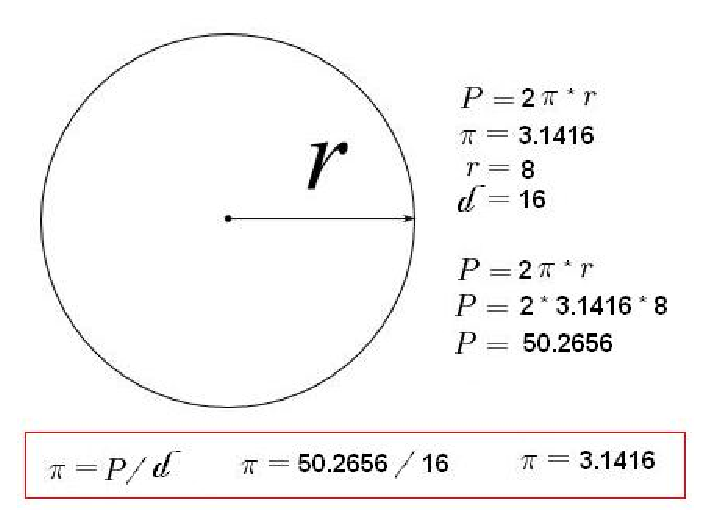
\includegraphics[width=0.75\textwidth]{pi1.eps}
\end{center}
\caption{Circunferencia de radio r}
\end{figure}


{\it\large El día 14 de marzo se celebra mundialmente el día de $\pi$, por ser su notación en algunos países, 3-14, una aproximación de dicho número.
Del número $\pi$ sabemos muchísimas cosas como que es irracional y trascendente, es protagonista de muchas fórmulas conocidas (como en áreas y volúmenes de figuras sencillas como la esfera), aparece en cuestiones relacionadas con probabilidad, está relacionado con el conjunto de Mandelbrot, forma parte de la identidad de Euler…
…pero también hay cosas que no sabemos: una de ellas, posiblemente la más importante es que no sabemos si el número $\pi$ es un número normal en base 10}
\end{abstract} 

\pagebreak

\section{Historia del cálculo de $\pi$}
El valor de $\pi$ se ha obtenido con diversas aproximaciones a lo largo de la historia, siendo una de las constantes matemáticas que más aparece en las ecuaciones de la física, junto con el número e.
La notación con la letra griega $\pi$ proviene de la inicial de las palabras de origen griego 'periferia' y 'perímetro' de un círculo, notación que fue utilizada primero por William Oughtred, cuyo uso fue propuesto por el matemático galés William Jones; aunque fue el matemático Leonhard Euler, con su obra 'Introducción al cálculo infinitesimal' quien la popularizó. Fue conocida anteriormente como constante de Ludolph (en honor al matemático Ludolph van Ceulen) o como constante de Arquímedes (que no se debe confundir con el número de Arquímedes).

La aproximación de arquímedes mediante polígonos regulares \cite{Ecamec} nos da como resultado los siguientes datos:

\begin{tabular}{ll}

Lados & Número Obtenido\\
\hline
36 & 3,1\\
360 & 3,141\\
3600 & 3,1415926\\
360000 & 3,141592653\\
3600000 & 3,14159265358\\
36000000 & 3,1415926535897\\
360000000 & 3,141592653589793\\
3600000000 & 3,14159265358979324

\end{tabular}


\subsection{Antiguo egipto}
El valor aproximado de $\Pi$ en las antiguas culturas se remonta a la época del escriba egipcio Ahmes en el año 1800 a. C., descrito en el papiro Rhind,3 donde se emplea un valor aproximado de $\Pi$ afirmando que el área de un círculo es similar a la de un cuadrado cuyo lado es igual al diámetro del círculo disminuido en 1/9; es decir, igual a 8/9 del diámetro. 
Entre los ocho documentos matemáticos hallados de la antigua cultura egipcia, en dos se habla de círculos. Uno es el papiro Rhind y el otro es el papiro de Moscú. Sólo en el primero se habla del valor aproximado del número $\Pi$. El investigador Otto Neugebauer, en un anexo de su libro The Exact Sciences in Antiquity,4 describe un método inspirado en los problemas del papiro de Ahmes para averiguar el valor de $\Pi$, mediante la aproximación del área de un cuadrado de lado 8, a la de un círculo de diámetro 8.

\subsection{Mesopotamia}
Algunos matemáticos mesopotámicos empleaban, en el cálculo de segmentos, valores de $\Pi$ igual a 3, alcanzando en algunos casos valores más aproximados, como el de:

\centerline{$\Pi \approx 3 + \frac{1}{8} = 3,125$} 

    
\section{Uso en matemáticas y otras ciencias}

A continuación se muestra un listado de las apariciones más importantes del número pi en diferentes entornos:

\begin{itemize}

\item Geometría y Trigonometría
Tal y como se muestra en 
\item Análisis Superior y Teoría de Números
\item Probabilidad y estadística.
Se puede calcular el numero pi mediante arroz y palillos \cite{Arroz}

\end{itemize}



\begin{thebibliography}{11}
\bibitem{Ecamec} www.ecamec.com/newsletter/notaa1209.html
\bibitem {Arroz} http://aprender-ensenyar-matematicas.blogspot.com.es/2012/02/vamos-ver-dos-formas-de-calcular-pi-en.html
\bibitem {Gaus} http://gaussianos.com/la-cuestion-mas-importante-que-aun-no-se-ha-respondido-sobre-el-numero-pi/
\bibitem {Wiki} http://es.wikipedia.org/wiki/N%C3%BAmero_%CF%80
\end{thebibliography}

\footnote{Facultad de Matemáticas. Técnicas Experimentales. Universidad de La Laguna}
\end{document}

